\chapter{Method}

\section{The PALSfit Bundle}

PALSfit is a Windows based software package, developed for the analysis of positron lifetime spectra, based on a non-linear least squares approach. Included are two modules, POSITRONFIT and RESOLUTIONFIT, which are used to deconvolve the lifetime components and resolution functions (respectively) from the lifetime spectra. As the scope of the project limited to lifetime component analysis, only the former will be used. PALSfit Version 3, or more simply PALSfit3, is the latest version of this package, which this project is aimed at evaluating. All subsequent references to "PALSfit" are to this specific version of the software.

Included with PALSfit is the PALSsim program, which generates lifetime spectra based on user input. PALSsim makes it possible to quickly generate spectra with full control over relevant parameters such as lifetimes, resolution function, background noise, etc. All spectra to be analysed in the project were produced using PALSsim.

\section{PALSsim}
\begin{figure}
    \centering
    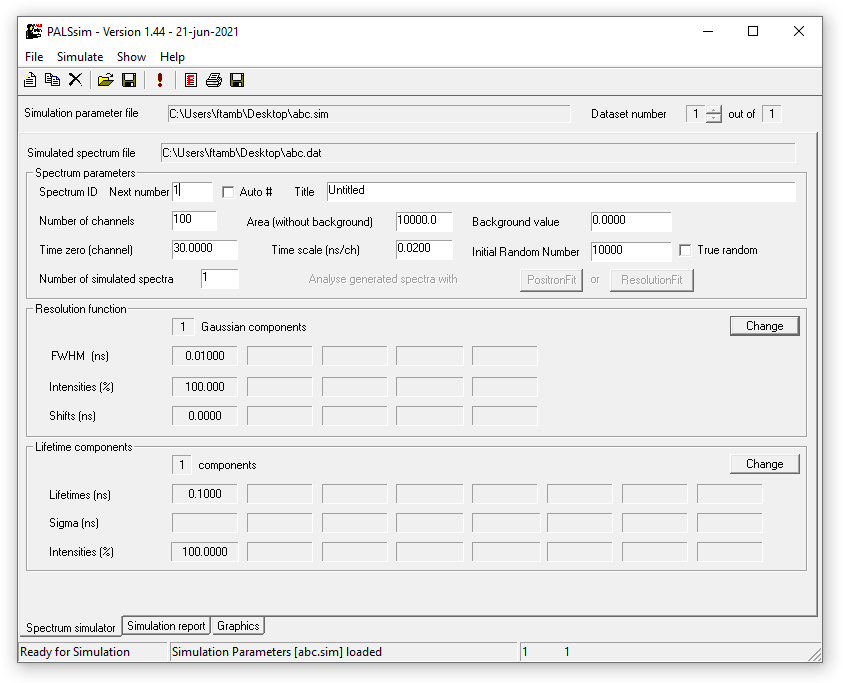
\includegraphics[width=0.8\linewidth]{PALSsim.PNG}
    \caption{PALSsim window}
    \label{fig:Psim}
\end{figure}

As can be seen in Fig.\ref{fig:Psim}, PALSsim groups user input data into three sections: Spectrum parameters, Resolution function and Lifetime components. A quick overview of each section, its associated parameters and the default values used in the project follows.

\subsection{Lifetime components}
In the \textit{Lifetime components} section, the number of components in the spectrum and their associated values can be modified. Only the \textit{Lifetimes} and \textit{Intensities} fields will be used for each component throughout this project, as we'll assume each lifetime component to be discrete. Up to eight components can be simulated, but the maximum number of components used in the project will be three.

\subsection{Resolution function}

The \textit{Resolution function} section deals with the instrument resolution function of the simulated spectrum. The resolution function is given by a sum of up to five Gaussian functions $G(t)$ with the width, relative height and peak position of each Gaussian component being controlled by the \textit{FWHM}, \textit{Intensities} and \textit{Shifts fields} respectively.

For the majority of this project, a three gaussian resolution function will be used, with the appropriate parameters taken from an experimental spectrum and indicated in Table \ref{tab:irfcomp}. For a visual representation of the IRF, see Fig. \ref{fig:irf}.

\vspace{0.7cm}

\begin{minipage}{0.6\textwidth}
    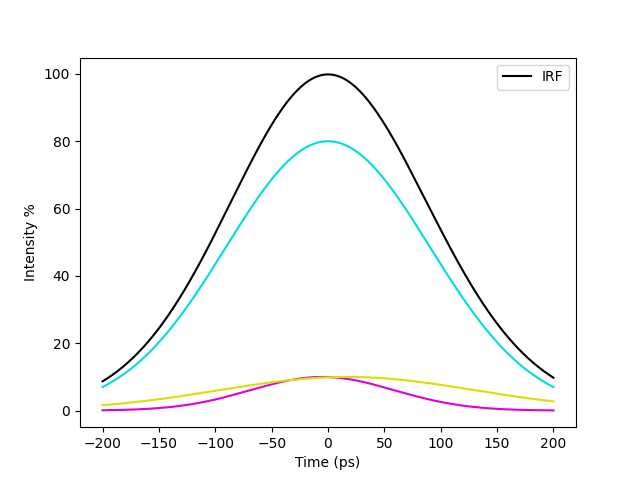
\includegraphics[width=\textwidth]{Batch 3/regular IRF/irf.png}
\end{minipage}
\begin{minipage}{0.35\textwidth}
    \centering
    \captionof{table}{IRF values}
    \label{tab:irfcomp}
    \begin{tabular}{|c|c|c|}
        \hline
        FWHM& Intensity& Shift \\
        (ps) & (\%) & (ps)\\
        \hline
        213.2 & 80 &  0\\
        150.2 & 10 & -5\\
        265.7 & 10 & 17\\
        \hline
    \end{tabular}
    \vspace{2.2cm}
    \captionof{figure}{Instrument Resolution Function}
    \label{fig:irf}
\end{minipage}


\subsection{Simulation parameters}

The variables found within the \textit{Simulation parameters} section affect the spectrum as a whole. Here we find parameters controlling the number of channels, time per channel, number of counts, $t_0$ and background noise. Relevant parameters and default values used are as follows:

\begin{itemize}
    \item Number of channels: 1000 
    \item Area (without background): 5650000 
    \item Background value: 8.5 
    \item Time zero (channel): 1400 
    \item Time scale (ps/ch): 5 
\end{itemize}
All other parameters were left unchanged.

\subsection{Generated files}

PALSsim generates five files every time a new spectrum is simulated. The file with the .dat extension contains the simulated spectrum, organized as a table of values for each channel. A .sim file stores the simulated values, allowing them to be reloaded into the program. A simulation report is generated every time a simulation is ran that contains data about the spectrum and saved in a .out file. Lastly two control files with the .pfc and .rfc extensions are generated to be read by PALSfit. Loading one or the other control file into PALSfit determines whether the POSITRONFIT or RESOLUTIONFIT module is used to analyse the spectrum (.pfc for the former and .rfc for the latter).

\section{PALSfit}

Opening a .pfc file, the spectrum and all relevant fitting values should be automatically loaded. Before fitting every spectrum in the project, the \textit{Spectrum setup} window was opened by clicking any of the two \textit{Change} buttons in the \textit{Spectrum} tab. Here the \textit{Default Ranges} button was clicked to ensure that the appropriate range was fitted and the spectrum was saved to the control file checking the relevant checkbox.

\begin{figure} [h]
    \centering
    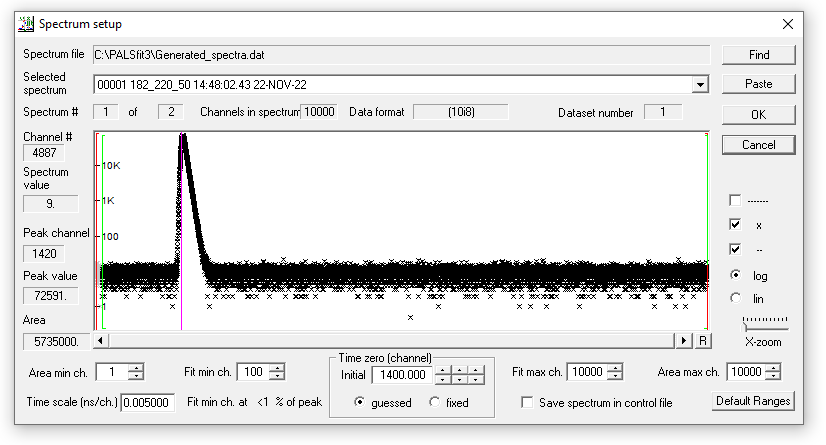
\includegraphics[width=0.63\linewidth]{SpecSetup.PNG}
    \caption{Spectrum setup window}
    \label{fig:SpecSet}
\end{figure}

A fit is performed by pressing the \textit{Analyse} button at the top of the window or pressing the F5 key. This generates a series of files in an output folder, contained in the same directory as the .pfc file. Of relevance are the .out file and .csv file that contain the results of the fit.

\section{Analysing fits}

Using PALSsim to generate spectra and PALSfit to fit those generated spectra, a series of trials were performed. Each trial 